\documentclass[11pt,a4paper]{article}
\usepackage[utf8]{inputenc}
\usepackage[T1]{fontenc}
\usepackage[dutch]{babel}
\usepackage{lmodern}
\usepackage{amsmath,amssymb,mathtools,bm}
\usepackage{geometry}
\usepackage{microtype}
\usepackage{enumitem}
\usepackage{booktabs}
\usepackage{array}
\usepackage{longtable}
\usepackage{hyperref}
\usepackage{xcolor}
\usepackage{tcolorbox}
\usepackage{fancyhdr}
\usepackage{titlesec}
\usepackage{setspace}
\usepackage{tikz}
\usetikzlibrary{arrows.meta,positioning,shapes.geometric}
\geometry{margin=2.3cm}
\setlength{\parindent}{0pt}
\setlength{\parskip}{0.6em}
\hypersetup{colorlinks=true,linkcolor=blue!55!black,urlcolor=blue!55!black}
\pagestyle{fancy}
\fancyhf{}
\lhead{Wiskunde Handboek}
\rhead{Fase 7}
\cfoot{\thepage}
\titleformat{\section}{\Large\bfseries}{\thesection}{0.6em}{}
\titleformat{\subsection}{\large\bfseries}{\thesubsection}{0.6em}{}
\newtcolorbox{kernidee}{colback=blue!4,colframe=blue!45!black,title=Kernidee}
\newtcolorbox{waarschuwing}{colback=yellow!8,colframe=yellow!45!black,title=Let op}
\newtcolorbox{voorbeeld}{colback=green!4,colframe=green!40!black,title=Voorbeeld}
\newtcolorbox{brug}{colback=purple!4,colframe=purple!45!black,title=Verbinding met eerdere fasen}
\newcommand{\dd}{\mathrm{d}}
\newcommand{\Tr}{\operatorname{Tr}}
\newcommand{\R}{\mathbb{R}}
\newcommand{\C}{\mathbb{C}}
\newcommand{\Lie}{\mathfrak{g}}

\begin{document}

\begin{titlepage}
\centering
\vspace*{2.2cm}
{\Huge\bfseries Cursus Fase 7\\[0.35cm] Differentiaalmeetkunde \& Kwantumvelden\par}
\vspace{1cm}
{\Large Van lokale geometrie naar gaugevelden en Yang--Mills\par}
\vfill
{\large Wiskunde Handboek\par}
\vspace{0.4cm}
{\large Eindfase van het leerpad\par}
\vspace*{2cm}
\end{titlepage}

\tableofcontents
\newpage

\section*{Inleiding}
\addcontentsline{toc}{section}{Inleiding}

Deze fase is het eindpunt van het leerpad. In de vorige fasen heb je getallen, algebra, functies, calculus, lineaire algebra, differentiaalvergelijkingen, complexe getallen, Fourier-analyse, groepentheorie, topologie en tensorrekening opgebouwd. In Fase 7 worden die onderdelen niet vervangen: ze worden samengebracht.

Het centrale thema is dat moderne fysica niet alleen vraagt \emph{welke grootheden bestaan}, maar ook \emph{hoe grootheden op verschillende punten met elkaar mogen worden vergeleken}, \emph{welke symmetrieën lokaal gelden} en \emph{hoe kromming uit zo'n lokale vergelijkingsregel ontstaat}.

De drie milestones uit het leerpad zijn:
\begin{enumerate}
    \item \textbf{7.1 Gevectoriseerde Bundels \& Connecties} --- de wiskundige beschrijving van gekromde ruimten en krachtenvelden;
    \item \textbf{7.2 Yang--Mills Theorie} --- de gauge-theoretische taal achter fundamentele interacties;
    \item \textbf{7.3 Het Begrip} --- de synthese: hoe geometrie, symmetrie, velden en kwantisatie in één raamwerk samenkomen.
\end{enumerate}

In standaard wiskundige terminologie spreken we meestal van \textbf{vectorbundels} in plaats van ``gevectoriseerde bundels''. Voor Yang--Mills is bovendien het begrip \textbf{principale bundel} belangrijk. Daarom behandelt deze cursus beide.

\begin{waarschuwing}
Deze cursus brengt je tot een degelijk conceptueel en technisch begrip van de klassieke geometrie van Yang--Mills en van de betekenis van de Mass Gap-vraag. Een volledig rigorieuze constructie van vierdimensionale kwantum-Yang--Mills-theorie met bewezen mass gap is geen afgerond onderdeel van de huidige wiskunde; dat is precies waarom het probleem zo fundamenteel is.
\end{waarschuwing}

\subsection*{Hoe je deze cursus gebruikt}
Werk in drie lagen:
\begin{enumerate}
    \item \textbf{Intuïtie:} probeer eerst te begrijpen welk probleem een nieuw object oplost.
    \item \textbf{Formalisme:} leer daarna de definitie en de notatie.
    \item \textbf{Toepassing:} verbind het begrip met geometrie, relativiteit of gauge-theorie.
\end{enumerate}

Bij elk nieuw symbool moet je jezelf twee vragen stellen: \emph{wat voor soort object is dit?} en \emph{op welke ruimte leeft het?} Dat voorkomt het merendeel van de verwarring in deze fase.

\section{Waar staan we in het leerpad?}

De essentie van Fase 6 was:
\[
\text{groep + topologie + tensor} \longrightarrow \text{structuur zonder afhankelijkheid van een gekozen voorstelling}.
\]

Fase 7 voegt één cruciaal idee toe: \textbf{lokale vergelijking}.

Een vector in het raakvlak $T_pM$ en een vector in $T_qM$ liggen in verschillende vectorruimten. Op een vlakke Euclidische ruimte merk je dat nauwelijks, omdat er een vanzelfsprekende manier lijkt te bestaan om pijlen te verschuiven. Op een algemene manifold bestaat zo'n vergelijking niet automatisch.

We hebben daarom een extra structuur nodig:
\[
\boxed{\text{connectie}}
\]

Een connectie vertelt hoe een vector, spinor of ander object langs de ruimte wordt ``meegenomen''. Zodra zo'n regel bestaat, kan men vragen of transport rond een gesloten lus het object terugbrengt naar zichzelf. Als dat niet zo is, meten we \textbf{kromming}.

Dat idee wordt twee keer gebruikt:
\begin{itemize}
    \item in differentiaalmeetkunde en algemene relativiteit: kromming van de ruimtetijd;
    \item in Yang--Mills-theorie: kromming van een interne gauge-bundel, geïnterpreteerd als veldsterkte.
\end{itemize}

\begin{kernidee}
De rode draad van Fase 7 is:
\[
\text{lokale ruimte} \to \text{bundel} \to \text{connectie} \to \text{parallel transport} \to \text{kromming} \to \text{veldsterkte}.
\]
\end{kernidee}

\newpage
\section{Milestone 7.1 --- Gevectoriseerde Bundels \& Connecties}

\subsection{Doelen van deze milestone}
Na dit hoofdstuk moet je kunnen uitleggen en gebruiken:
\begin{itemize}
    \item manifolds, kaarten en lokale coördinaten;
    \item raakruimten $T_pM$ en vectorvelden;
    \item differentiaalvormen en de uitwendige afgeleide $\dd$;
    \item vectorbundels en secties;
    \item principale $G$-bundels en geassocieerde vectorbundels;
    \item connecties, covariante afgeleiden en parallel transport;
    \item metriek, Levi-Civita-connectie en Christoffelsymbolen;
    \item kromming, holonomie en de relatie tussen connectie en veldsterkte.
\end{itemize}

\subsection{Van een oppervlak naar een manifold}

Een manifold is een ruimte die lokaal op gewone Euclidische ruimte lijkt. De aarde is een intuïtief voorbeeld: globaal is haar oppervlak gekromd, maar op een voldoende klein gebied kan men een vlakke kaart gebruiken.

Formeel is een $n$-dimensionale gladde manifold $M$ een topologische ruimte die lokaal beschreven kan worden door kaarten
\[
\varphi: U \subset M \longrightarrow \varphi(U) \subset \R^n,
\]
waarbij overgangsfuncties tussen overlappende kaarten voldoende glad zijn.

Een kaart geeft aan een punt $p\in M$ coördinaten
\[
(x^1,\dots,x^n).
\]
Die coördinaten zijn niet het punt zelf. Ze zijn alleen een beschrijving.

\begin{brug}
Dit is dezelfde filosofie als bij vectoren en tensoren in Fase 6: componenten hangen af van de gekozen basis of coördinaten, maar het geometrische object zelf niet.
\end{brug}

\subsection{Raakvectoren en de raakruimte}

Op een gekromde manifold kan een vector niet simpelweg als een pijl ``in de omgevende ruimte'' worden gedefinieerd, want een abstracte manifold hoeft zelfs niet in een grotere Euclidische ruimte ingebed te zijn.

Een intrinsieke definitie gebruikt afgeleiden. Een raakvector $v\in T_pM$ kan worden opgevat als een lineaire operator die op gladde functies $f$ werkt en voldoet aan de productregel:
\[
v(fg)=v(f)g(p)+f(p)v(g).
\]

In lokale coördinaten heeft iedere raakvector de vorm
\[
v=v^\mu\frac{\partial}{\partial x^\mu}\Big|_p.
\]

De verzameling van alle raakvectoren in $p$ vormt de \textbf{raakruimte} $T_pM$.

Voor ieder punt hebben we dus een andere vectorruimte:
\[
p\mapsto T_pM.
\]

\subsection{De raakbundel}

Door alle raakruimten samen te nemen krijgen we de \textbf{raakbundel}
\[
TM=\bigcup_{p\in M}T_pM.
\]

Er is een natuurlijke projectie
\[
\pi:TM\to M,
\qquad
\pi(v_p)=p.
\]

De ruimte $M$ heet de \textbf{basisruimte}; $T_pM$ heet de \textbf{fiber} boven $p$.

Een vectorveld is dan een keuze van één raakvector boven elk punt:
\[
X:p\mapsto X_p\in T_pM.
\]
Formeel is een vectorveld een sectie $X:M\to TM$ met
\[
\pi\circ X=\operatorname{id}_M.
\]

\subsection{Algemene vectorbundels}

De raakbundel is één voorbeeld van een algemener object.

Een rang-$k$ vectorbundel bestaat uit:
\begin{itemize}
    \item een totale ruimte $E$;
    \item een basismanifold $M$;
    \item een projectie $\pi:E\to M$;
    \item voor ieder $p\in M$ een vectorruimte $E_p=\pi^{-1}(p)$ van dimensie $k$;
    \item lokale gebieden waarin de bundel eruitziet als een product $U\times\R^k$ of $U\times\C^k$.
\end{itemize}

Lokaal is de bundel eenvoudig; globaal kan hij verdraaid zijn.

\begin{voorbeeld}
De Möbiusband kan als een eenvoudige reële lijnbundel boven de cirkel worden gezien. Lokaal lijkt iedere fiber op een rechte lijn, maar na één omwenteling is de oriëntatie omgekeerd. Dit toont dat ``lokaal product'' niet ``globaal product'' hoeft te betekenen.
\end{voorbeeld}

\subsection{Secties}

Een sectie van een bundel kiest in iedere fiber één element:
\[
s:M\to E,
\qquad
s(p)\in E_p.
\]

Veel fysische velden zijn precies zulke secties:
\begin{itemize}
    \item een vectorveld is een sectie van $TM$;
    \item een covectorveld is een sectie van $T^*M$;
    \item een tensorveld is een sectie van een tensorbundel;
    \item een materieveld in gauge-theorie kan een sectie zijn van een geassocieerde vectorbundel.
\end{itemize}

\subsection{Covectoren en differentiaalvormen}

De duale ruimte $T_p^*M$ bestaat uit lineaire afbeeldingen van $T_pM$ naar $\R$ of $\C$. Een 1-vorm is een covectorveld.

Als $f$ een gladde functie is, dan is zijn differentiaal
\[
\dd f
\]
een 1-vorm. In lokale coördinaten:
\[
\dd f=\frac{\partial f}{\partial x^\mu}\dd x^\mu.
\]

Meer algemeen is een $p$-vorm een antisymmetrische covariante tensor van rang $p$.

Een 2-vorm heeft lokaal de vorm
\[
\omega=\frac12\omega_{\mu\nu}\,\dd x^\mu\wedge\dd x^\nu,
\]
met
\[
\omega_{\mu\nu}=-\omega_{\nu\mu}.
\]

\subsection{Het wedge-product}

Het symbool $\wedge$ is het uitwendige product. Voor 1-vormen geldt
\[
\alpha\wedge\beta=-\beta\wedge\alpha.
\]
Daarom is
\[
\alpha\wedge\alpha=0.
\]

Voor basisvormen:
\[
\dd x^\mu\wedge\dd x^\nu=-\dd x^\nu\wedge\dd x^\mu.
\]

Deze antisymmetrie is precies wat we nodig hebben voor oppervlakte-elementen, fluxen en veldsterkten.

\subsection{De uitwendige afgeleide}

De uitwendige afgeleide
\[
\dd:\Omega^p(M)\to\Omega^{p+1}(M)
\]
verhoogt de graad van een vorm met één.

Voor een functie $f$:
\[
\dd f=\partial_\mu f\,\dd x^\mu.
\]

Voor een 1-vorm $A=A_\mu\dd x^\mu$:
\[
\dd A=\frac12(\partial_\mu A_\nu-\partial_\nu A_\mu)\dd x^\mu\wedge\dd x^\nu.
\]

Een fundamentele eigenschap is
\[
\boxed{\dd^2=0}.
\]

Dat betekent bijvoorbeeld $\dd(\dd f)=0$.

\subsection{Waarom differentiaalvormen zo krachtig zijn}

Differentiaalvormen zijn natuurlijke integratieobjecten:
\begin{itemize}
    \item 1-vormen over krommen;
    \item 2-vormen over oppervlakken;
    \item 3-vormen over volumes;
    \item $n$-vormen over $n$-dimensionale manifolds.
\end{itemize}

De algemene Stokes-stelling luidt:
\[
\int_{\partial\Omega}\omega=\int_{\Omega}\dd\omega.
\]

Dit omvat als speciale gevallen de hoofdstelling van calculus, de stelling van Green, Gauss en de klassieke Stokes-stelling.

\subsection{De metriek}

Een metriek is een symmetrisch $(0,2)$-tensorveld
\[
g=g_{\mu\nu}\,\dd x^\mu\otimes\dd x^\nu.
\]

Ze definieert een lokaal inproduct:
\[
g_p:T_pM\times T_pM\to\R.
\]

De infinitesimale afstand wordt geschreven als
\[
\dd s^2=g_{\mu\nu}\dd x^\mu\dd x^\nu.
\]

In Euclidische ruimte is $g_{ij}=\delta_{ij}$. In de ruimtetijd kan de metriek Lorentz-signatuur hebben, bijvoorbeeld $(-,+,+,+)$.

Met de metriek kan men indices verlagen en verhogen:
\[
v_\mu=g_{\mu\nu}v^\nu,
\qquad
v^\mu=g^{\mu\nu}v_\nu.
\]

\subsection{Waarom gewone afgeleiden niet volstaan}

Neem een vectorveld
\[
V=V^\mu\partial_\mu.
\]
De componenten $V^\mu$ veranderen onder een coördinatenwisseling, maar ook de basisvectoren $\partial_\mu$ veranderen. Als je alleen $\partial_\nu V^\mu$ neemt, negeer je de verandering van de basis.

Daarom transformeert een gewone partiële afgeleide van vectorcomponenten in het algemeen niet als een tensor.

We introduceren een \textbf{covariante afgeleide}:
\[
\nabla_\mu V^\nu=\partial_\mu V^\nu+\Gamma^{\nu}{}_{\mu\rho}V^\rho.
\]

Voor een covector:
\[
\nabla_\mu \omega_\nu=\partial_\mu\omega_\nu-\Gamma^{\rho}{}_{\mu\nu}\omega_\rho.
\]

Het extra teken weerspiegelt het duale transformatiegedrag.

\subsection{Christoffelsymbolen}

Voor de Levi-Civita-connectie zijn de Christoffelsymbolen
\[
\Gamma^\rho{}_{\mu\nu}
=\frac12g^{\rho\sigma}
\left(
\partial_\mu g_{\sigma\nu}
+\partial_\nu g_{\sigma\mu}
-\partial_\sigma g_{\mu\nu}
\right).
\]

Ze zijn afgeleid uit de metriek wanneer we twee eisen opleggen:
\begin{enumerate}
    \item metriekcompatibiliteit: $\nabla_\rho g_{\mu\nu}=0$;
    \item torsievrijheid: $\Gamma^\rho{}_{\mu\nu}=\Gamma^\rho{}_{\nu\mu}$.
\end{enumerate}

\begin{waarschuwing}
Christoffelsymbolen zijn geen tensorcomponenten. In geschikte coördinaten kunnen ze in één punt verdwijnen, zelfs wanneer de kromming daar niet nul is. Kromming is dus fundamenteler dan de Christoffelsymbolen zelf.
\end{waarschuwing}

\subsection{Geodeten}

Een geodeet is een kromme die zijn eigen raakvector parallel transporteert:
\[
\nabla_{\dot\gamma}\dot\gamma=0.
\]

In coördinaten:
\[
\frac{\dd^2x^\rho}{\dd\lambda^2}
+\Gamma^\rho{}_{\mu\nu}
\frac{\dd x^\mu}{\dd\lambda}
\frac{\dd x^\nu}{\dd\lambda}=0.
\]

In vlakke ruimte zijn geodeten rechte lijnen. Op een bol zijn grootcirkels voorbeelden van geodeten.

\subsection{Parallel transport}

Parallel transport is de concrete betekenis van een connectie. Een vector $V$ wordt langs een kromme $\gamma$ parallel getransporteerd als
\[
\nabla_{\dot\gamma}V=0.
\]

Op een gekromd oppervlak kan een vector na transport rond een gesloten lus in een andere richting terugkomen. Dat verschil is geometrische informatie.

\subsection{Kromming uit niet-commuterende afgeleiden}

De Riemann-kromming meet het niet-commuteren van covariante afgeleiden:
\[
[\nabla_\mu,\nabla_\nu]V^\rho
=R^\rho{}_{\sigma\mu\nu}V^\sigma
\]
voor een torsievrije connectie in een coördinatenbasis.

De componenten zijn
\[
R^\rho{}_{\sigma\mu\nu}
=\partial_\mu\Gamma^\rho{}_{\nu\sigma}
-\partial_\nu\Gamma^\rho{}_{\mu\sigma}
+\Gamma^\rho{}_{\mu\lambda}\Gamma^\lambda{}_{\nu\sigma}
-\Gamma^\rho{}_{\nu\lambda}\Gamma^\lambda{}_{\mu\sigma}.
\]

Contracties leveren:
\[
R_{\mu\nu}=R^\rho{}_{\mu\rho\nu}
\]
en
\[
R=g^{\mu\nu}R_{\mu\nu}.
\]

Dit zijn respectievelijk de Ricci-tensor en de scalaire kromming.

\subsection{Torsie}

Voor vectorvelden $X,Y$ definieert men de torsie van een connectie als
\[
T(X,Y)=\nabla_XY-\nabla_YX-[X,Y].
\]

De Levi-Civita-connectie heeft $T=0$. Andere geometrische theorieën kunnen wel torsie toelaten.

\subsection{Principale bundels}

Voor Yang--Mills is een gewone vectorbundel niet de meest fundamentele constructie. De natuurlijke geometrische drager van gauge-symmetrie is een \textbf{principale $G$-bundel}
\[
\pi:P\to M,
\]
waarbij een Lie-groep $G$ op de fibers werkt.

Intuïtief bevat elke fiber boven $p$ alle mogelijke lokale ``gauge-frames'' die via elementen van $G$ met elkaar samenhangen.

Lokaal lijkt
\[
P|_U\cong U\times G.
\]
Globaal kan de bundel niet-triviaal zijn.

\subsection{Geassocieerde vectorbundels}

Als $G$ op een vectorruimte $V$ werkt via een representatie
\[
\rho:G\to GL(V),
\]
kan uit een principale bundel een vectorbundel worden opgebouwd:
\[
E=P\times_G V.
\]

Materievelden kunnen dan als secties van $E$ worden gezien.

Dit levert het conceptuele schema:
\[
\boxed{
\text{principale bundel }P
\;\xrightarrow{\text{representatie}}\;
\text{geassocieerde vectorbundel }E
}
\]

\subsection{Een connectie op een gauge-bundel}

Lokaal wordt een gauge-connectie voorgesteld door een Lie-algebra-waardige 1-vorm
\[
A=A_\mu\dd x^\mu,
\qquad A_\mu\in\Lie.
\]

Hier is $\Lie$ de Lie-algebra van de gaugegroep $G$.

Voor een materieveld $\psi$ in een representatie van $G$ wordt de gewone afgeleide vervangen door een gauge-covariante afgeleide:
\[
D\psi=(\dd+A)\psi,
\]
of, afhankelijk van conventies,
\[
D_\mu=\partial_\mu+igA_\mu.
\]

De factor $i$ en koppeling $g$ zijn conventie- en representatieafhankelijk.

\subsection{Kromming van een gauge-connectie}

De kromming van $A$ is de 2-vorm
\[
\boxed{F=\dd A+A\wedge A.}
\]

In componenten:
\[
F_{\mu\nu}
=\partial_\mu A_\nu-\partial_\nu A_\mu+[A_\mu,A_\nu].
\]
Met een expliciete koppeling kan de laatste term bijvoorbeeld $ig[A_\mu,A_\nu]$ bevatten.

Voor een abelse groep zoals $U(1)$ commuteert de Lie-algebra en verdwijnt de commutatorterm. Dan:
\[
F=\dd A.
\]

Voor niet-abelse groepen zoals $SU(2)$ en $SU(3)$ blijft de zelfinteractieterm bestaan.

\subsection{Holonomie}

Transport rond een gesloten lus $\gamma$ wordt beschreven door de holonomie. In gauge-theorie verschijnt de padgeordende exponentiële:
\[
U_\gamma=\mathcal{P}\exp\left(-\int_\gamma A\right).
\]

Kromming kan worden gezien als de infinitesimale versie van niet-triviale holonomie.

\begin{kernidee}
Een connectie vertelt hoe je lokaal vergelijkt. Kromming meet de inconsistentie die verschijnt wanneer je rond een lus vergelijkt. In Yang--Mills wordt die kromming fysisch geïnterpreteerd als veldsterkte.
\end{kernidee}

\subsection{De Hodge-ster}

Op een georiënteerde manifold met metriek zet de Hodge-ster $p$-vormen om in $(n-p)$-vormen:
\[
*:\Omega^p(M)\to\Omega^{n-p}(M).
\]

Daardoor kan men een natuurlijke scalairachtige integraal van veldsterkten bouwen:
\[
\Tr(F\wedge *F).
\]

Dit wordt straks de elegante differentiaalvorm-notatie van de Yang--Mills-actie.

\subsection{Milestone 7.1 --- oefeningen}

\begin{enumerate}
\item Leg in eigen woorden uit waarom een manifold lokaal maar niet noodzakelijk globaal op $\R^n$ lijkt.
\item Wat is het verschil tussen $T_pM$ en $TM$?
\item Waarom is een vectorveld een sectie van $TM$?
\item Wat is de fiber van de cotangentbundel $T^*M$ boven $p$?
\item Waarom is een 2-vorm antisymmetrisch?
\item Toon uit antisymmetrie dat $\alpha\wedge\alpha=0$ voor een 1-vorm $\alpha$.
\item Wat betekent $\dd^2=0$ conceptueel?
\item Waarom transformeert $\partial_\mu V^\nu$ niet vanzelf als een tensor?
\item Welke rol speelt $\Gamma^\rho{}_{\mu\nu}$ in $\nabla_\mu V^\rho$?
\item Welke twee eigenschappen karakteriseren de Levi-Civita-connectie?
\item Wat betekent parallel transport?
\item Waarom kan transport rond een lus informatie over kromming geven?
\item Schrijf de geodetische vergelijking op.
\item Wat meet de Riemann-tensor?
\item Wat is het verschil tussen een vectorbundel en een principale bundel?
\item Waarom heb je een representatie $\rho:G\to GL(V)$ nodig om een geassocieerde vectorbundel te bouwen?
\item Wat voor soort object is $A$ lokaal in gauge-theorie?
\item Wat voor soort object is $F$?
\item Waarom verdwijnt $A\wedge A$ effectief in een $U(1)$-theorie?
\item Wat is de betekenis van de Hodge-ster in de Yang--Mills-actie?
\end{enumerate}

\subsection*{Antwoorden 7.1}
\begin{enumerate}
\item Omdat elke kleine omgeving via een kaart met een open deel van $\R^n$ kan worden geïdentificeerd, terwijl de globale topologie of kromming daarvan kan afwijken.
\item $T_pM$ is één raakruimte boven één punt; $TM$ is de verzameling van alle raakruimten samen.
\item Omdat het in ieder punt $p$ één vector $X_p\in T_pM$ kiest.
\item $T_p^*M$, de duale ruimte van $T_pM$.
\item Omdat wisselen van twee argumenten het teken omkeert.
\item $\alpha\wedge\alpha=-\alpha\wedge\alpha$, dus in karakteristiek nul volgt $2\alpha\wedge\alpha=0$ en daarmee $\alpha\wedge\alpha=0$.
\item Dat een uitwendige afgeleide van iets dat al exact als $\dd$ van iets is ontstaan, nul is; lokaal is ``grens van grens'' nul.
\item Omdat bij een coördinatenwisseling ook de lokale basis verandert; de gewone afgeleide corrigeert die verandering niet.
\item Het compenseert de verandering van de basis en definieert de connectie in lokale coördinaten.
\item Metriekcompatibiliteit en torsievrijheid.
\item Een regel om een geometrisch object langs een kromme te vergelijken zonder het volgens de connectie ``te draaien''.
\item Omdat het eindresultaat kan afhangen van het gevolgde pad; de infinitesimale afwijking wordt door de kromming gemeten.
\item $\dd^2x^\rho/\dd\lambda^2+\Gamma^\rho{}_{\mu\nu}(\dd x^\mu/\dd\lambda)(\dd x^\nu/\dd\lambda)=0$.
\item Het niet-commuteren van covariante afgeleiden, of equivalent de infinitesimale path-afhankelijkheid van parallel transport.
\item Een vectorbundel heeft vectorruimten als fibers; een principale $G$-bundel heeft de groep $G$ als structurele fiber met een vrije groepactie.
\item Omdat de groep moet weten hoe zij op de vectorruimte $V$ werkt.
\item Een Lie-algebra-waardige 1-vorm: de lokale representatie van een connectie.
\item Een Lie-algebra-waardige 2-vorm: de kromming of veldsterkte.
\item Omdat de Lie-algebra abels is, zodat de commutator nul is.
\item Ze zet de 2-vorm $F$ om in een complementaire vorm zodat $F\wedge *F$ een topvorm wordt die over de ruimtetijd kan worden geïntegreerd.
\end{enumerate}

\newpage
\section{Milestone 7.2 --- Yang--Mills Theorie}

\subsection{Doelen van deze milestone}
Na dit hoofdstuk moet je kunnen uitleggen:
\begin{itemize}
    \item het verschil tussen globale en lokale symmetrie;
    \item waarom lokaliseren van een symmetrie een connectie vereist;
    \item de rol van Lie-groepen $U(1)$, $SU(2)$ en $SU(3)$;
    \item representaties en generatoren;
    \item de veldsterkte $F$ als kromming;
    \item de Yang--Mills-actie en de klassieke veldvergelijkingen;
    \item gauge-transformaties en gauge-invariantie;
    \item Wilson-lussen en holonomie;
    \item de overgang van klassiek naar kwantum;
    \item de betekenis van de Mass Gap-vraag.
\end{itemize}

\subsection{Van globale naar lokale symmetrie}

Beschouw een complex veld $\psi(x)$ en een globale faseverandering
\[
\psi(x)\mapsto e^{i\alpha}\psi(x),
\]
waar $\alpha$ overal dezelfde constante is.

De gewone afgeleide transformeert netjes:
\[
\partial_\mu\psi\mapsto e^{i\alpha}\partial_\mu\psi.
\]

Maak de fase nu lokaal:
\[
\psi(x)\mapsto e^{i\alpha(x)}\psi(x).
\]
Dan ontstaat
\[
\partial_\mu(e^{i\alpha(x)}\psi)
=e^{i\alpha(x)}\left(\partial_\mu\psi+i(\partial_\mu\alpha)\psi\right).
\]

De extra term $(\partial_\mu\alpha)\psi$ verbreekt de eenvoudige covariantie.

De oplossing is een nieuwe grootheid $A_\mu$ invoeren en definiëren
\[
D_\mu=\partial_\mu+igA_\mu
\]
zodat $D_\mu\psi$ op dezelfde manier transformeert als $\psi$.

\begin{kernidee}
Een lokaal gekozen symmetrieframe kan van punt tot punt veranderen. De gauge-connectie registreert hoe die lokale frames met elkaar vergeleken moeten worden.
\end{kernidee}

\subsection{Gaugegroep en Lie-algebra}

Een Yang--Mills-theorie kiest een compacte Lie-groep $G$ als gaugegroep. Belangrijke voorbeelden zijn:
\[
U(1),\qquad SU(2),\qquad SU(3).
\]

De Lie-algebra $\Lie$ bestaat uit generatoren van infinitesimale transformaties. Kies een basis $T^a$. Dan gelden commutatierelaties
\[
[T^a,T^b]=if^{ab}{}_cT^c
\]
in een veelgebruikte conventie.

De getallen $f^{ab}{}_c$ zijn de structuurconstanten.

Voor een abelse algebra zijn alle commutatoren nul. Voor een niet-abelse algebra niet.

\subsection{Representaties}

Een symmetrie werkt pas op een fysisch veld nadat een representatie is gekozen. Een materieveld kan bijvoorbeeld transformeren als
\[
\psi\mapsto U(x)\psi,
\qquad U(x)\in G.
\]

Dezelfde abstracte groep kan verschillende representaties hebben. Dat is fysisch belangrijk: verschillende deeltjesvelden kunnen verschillende ``ladingen'' of transformatie-eigenschappen dragen.

\subsection{De gaugepotentiaal}

Schrijf lokaal
\[
A_\mu=A_\mu^aT^a.
\]

De index $\mu$ is een ruimtetijdindex; de index $a$ is een interne Lie-algebra-index.

Dit onderscheid is fundamenteel:
\begin{itemize}
    \item $\mu$ vertelt in welke richting in de ruimtetijd;
    \item $a$ vertelt in welke richting in de interne symmetrieruimte.
\end{itemize}

\subsection{Gauge-transformatie van de connectie}

Onder een lokale transformatie $U(x)$ verandert de connectie schematisch als
\[
A\mapsto UAU^{-1}-\dd U\,U^{-1},
\]
waar conventies tekens en factoren $i/g$ kunnen veranderen.

De inhomogene term met $\dd U$ is precies wat nodig is om de afgeleide van $U(x)$ te compenseren.

De kromming transformeert eenvoudiger:
\[
F\mapsto UFU^{-1}.
\]

Daarom kan een spoor zoals
\[
\Tr(F_{\mu\nu}F^{\mu\nu})
\]
gauge-invariant zijn.

\subsection{Veldsterkte als kromming}

De definitie
\[
F=\dd A+A\wedge A
\]
is exact analoog aan het krommingsidee van de vorige milestone.

In componenten, met een gebruikelijke conventie:
\[
F^a_{\mu\nu}
=\partial_\mu A^a_\nu-\partial_\nu A^a_\mu
+g f^{a}{}_{bc}A^b_\mu A^c_\nu.
\]

De laatste term is typisch niet-abels. Daardoor kan het gaugeveld met zichzelf interageren.

\subsection{$U(1)$ als abelse limiet}

Voor elektromagnetisme is de gaugegroep $U(1)$. Omdat de algebra abels is,
\[
[A_\mu,A_\nu]=0.
\]
Dus
\[
F_{\mu\nu}=\partial_\mu A_\nu-\partial_\nu A_\mu.
\]

Dit is de relativistische elektromagnetische veldtensor.

Yang--Mills generaliseert dit naar niet-commuterende interne symmetrieën.

\subsection{De Yang--Mills-actie}

In componentnotatie is de klassieke actie in vier dimensies schematisch
\[
S_{\mathrm{YM}}=-\frac14\int \dd^4x\,F^a_{\mu\nu}F^{a\mu\nu},
\]
waar normalisaties afhangen van conventie.

In geometrische notatie:
\[
\boxed{S_{\mathrm{YM}}\propto \int_M \Tr(F\wedge *F).}
\]

Deze formule is compact omdat ze verschillende ideeën tegelijk bevat:
\begin{itemize}
    \item $F$: kromming van de gauge-connectie;
    \item $*$: de metrische structuur van de ruimtetijd;
    \item $\wedge$: combinatie tot een integreerbare topvorm;
    \item $\Tr$: een invariant in de interne Lie-algebra.
\end{itemize}

\subsection{Het variatieprincipe}

Zoals in klassieke mechanica worden de veldvergelijkingen gevonden door de actie stationair te maken:
\[
\delta S=0.
\]

Variëren van $A$ levert in vacuüm
\[
\boxed{D_\mu F^{\mu\nu}=0.}
\]

Met materiebronnen verschijnt schematisch
\[
D_\mu F^{\mu\nu}=J^\nu.
\]

Hier is $D_\mu$ zelf gauge-covariant.

\subsection{Bianchi-identiteit}

De kromming voldoet aan
\[
\boxed{DF=0.}
\]

In componenten:
\[
D_{[\mu}F_{\nu\rho]}=0.
\]

Dit is de gauge-theoretische analogie van een geometrische identiteit voor kromming.

\subsection{Noether en symmetrie}

In Fase 6 leerde je symmetrie als groepstructuur kennen. In veldentheorie krijgt symmetrie een dynamische rol.

Een continue \emph{globale} symmetrie leidt via de eerste stelling van Noether tot een behouden stroom. Lokale gauge-symmetrie is subtieler: zij bevat redundantie in onze beschrijving. De bijbehorende identiteiten horen bij Noethers tweede stelling.

\begin{waarschuwing}
Een gauge-transformatie moet niet zonder meer worden geïnterpreteerd als een verandering naar een fysisch andere toestand. Vaak beschrijft zij dezelfde fysische configuratie in een andere lokale gauge.
\end{waarschuwing}

\subsection{Wilson-lussen}

Voor een gesloten kromme $C$ definieert men een Wilson-lus
\[
W(C)=\Tr\,\mathcal{P}\exp\left(i g\oint_C A\right).
\]

Dit object meet gauge-invariante informatie over holonomie langs de lus.

In niet-perturbatieve gauge-theorie spelen Wilson-lussen een centrale rol, onder meer bij de studie van confinering.

\subsection{Het standaardmodel als gauge-theorie}

De gaugegroep van het standaardmodel is
\[
SU(3)_C\times SU(2)_L\times U(1)_Y.
\]

Schematisch:
\begin{itemize}
    \item $SU(3)_C$: sterke interactie, quantumchromodynamica;
    \item $SU(2)_L\times U(1)_Y$: electroweakke theorie;
    \item na spontane symmetriebreking verschijnen elektromagnetisme en de massieve $W^\pm$- en $Z$-bosonen.
\end{itemize}

Yang--Mills is dus geen afzonderlijke kracht, maar het algemene gauge-theoretische raamwerk waarin deze interacties worden geformuleerd.

\subsection{Waarom niet-abelse theorieën moeilijker zijn}

In een abelse theorie is $F$ lineair in $A$. In een niet-abelse theorie bevat $F$ termen kwadratisch in $A$. De actie bevat daardoor hogere machten van $A$ en dus zelfinteracties.

Dat leidt tot:
\begin{itemize}
    \item complexere klassieke oplossingen;
    \item niet-lineaire veldvergelijkingen;
    \item rijkere topologie;
    \item sterke niet-perturbatieve effecten;
    \item grote technische moeilijkheden bij kwantisatie.
\end{itemize}

\subsection{Topologische sectoren}

Omdat gaugevelden op bundels leven, kan de globale topologie van de bundel fysische betekenis krijgen. Niet alle configuraties hoeven continu in elkaar vervormbaar te zijn.

Voor geschikte theorieën verschijnen topologische grootheden zoals karakteristieke klassen en instantongetallen. Conceptueel is dit het moment waarop Fase 6-topologie terugkeert als onderdeel van veldentheorie.

\subsection{Van klassieke naar kwantum-Yang--Mills}

Klassiek is $A_\mu^a(x)$ een veldconfiguratie die aan veldvergelijkingen voldoet. In kwantumveldentheorie worden amplitudes verbonden aan fluctuaties van velden.

Een formele padintegraalnotatie is
\[
Z=\int \mathcal{D}A\;e^{\frac{i}{\hbar}S[A]}.
\]

In Euclidische tijd verschijnt vaak
\[
Z_E=\int \mathcal{D}A\;e^{-S_E[A]/\hbar}.
\]

Deze uitdrukkingen zijn buiten eenvoudige gevallen geen gewone eindig-dimensionale integralen. Ze vereisen regularisatie, renormalisatie en zorgvuldige definitie.

\subsection{Gauge-fixing}

Omdat veel $A$-configuraties dezelfde fysische toestand kunnen vertegenwoordigen, telt een naïeve padintegraal gauge-equivalente configuraties herhaaldelijk mee.

Daarom kiest men een gauge-conditie, bijvoorbeeld in een lokale perturbatieve behandeling
\[
\partial_\mu A^\mu=0,
\]
en corrigeert men de maat. In niet-abelse theorie leidt dit tot Faddeev--Popov-determinanten en ghostvelden.

Ghostvelden zijn geen gewone waarneembare deeltjes; ze coderen de wiskundige correctie die nodig is voor de gauge-redundantie in perturbatieve kwantisatie.

\subsection{Renormalisatie en schaalafhankelijkheid}

Kwantumveldentheorie bevat bijdragen van zeer hoge impulsen. Bij renormalisatie wordt de relatie tussen gemeten parameters en de beschrijving op een gekozen energieschaal systematisch geregeld.

In niet-abelse Yang--Mills-theorie kan de effectieve koppeling met schaal veranderen. Voor QCD leidt dit tot \textbf{asymptotische vrijheid}: op zeer hoge energieën wordt de sterke koppeling zwakker.

Bij lage energie wordt de koppeling sterk, waardoor perturbatietheorie faalt en niet-perturbatieve methoden noodzakelijk worden.

\subsection{Confinering}

In QCD worden quarks en gluonen niet als geïsoleerde asymptotische deeltjes waargenomen. Ze verschijnen gebonden in hadronen.

Confinering is nauw verbonden met de sterke, niet-perturbatieve dynamica van de theorie. Wilson-lussen leveren een nuttige diagnostiek: een zogenoemde area law is een klassieke indicator van confinering in geschikte regimes.

\subsection{Wat is een mass gap?}

Laat de vacuümenergie $E_0$ zijn. Een mass gap betekent dat de eerstvolgende fysische excitatie een strikt positieve minimale energie boven het vacuüm heeft:
\[
\Delta=E_1-E_0>0.
\]

In een relativistische theorie vertaalt zo'n energieschaal zich in een positieve massaschaal voor de lichtste excitatie.

Het verrassende in pure klassieke Yang--Mills is dat de fundamentele Lagrangiaan in vier dimensies geen expliciete massaterm nodig heeft. Kwantumdynamica kan toch een eigen massaschaal genereren. Dit heet \textbf{dimensional transmutation}.

\subsection{Waarom de Mass Gap-vraag diep is}

De moeilijkheid is niet alleen ``bereken de massa van een deeltje''. Men wil een mathematisch consistente vierdimensionale quantum-Yang--Mills-theorie construeren en vervolgens bewijzen dat haar spectrum boven het vacuüm een positieve kloof bezit.

Daarvoor moeten tegelijk problemen rond:
\begin{itemize}
    \item oneindig-dimensionale veldruimten;
    \item gauge-redundantie;
    \item renormalisatie;
    \item niet-perturbatieve dynamica;
    \item spectraaltheorie;
    \item functionaalanalyse;
    \item globale geometrie en topologie
\end{itemize}
worden beheerst.

\subsection{Milestone 7.2 --- oefeningen}

\begin{enumerate}
\item Waarom werkt een constante faseverandering eenvoudiger dan een lokale faseverandering?
\item Welke extra term ontstaat wanneer $\alpha=\alpha(x)$ in $\partial_\mu(e^{i\alpha(x)}\psi)$?
\item Waarom introduceert men $A_\mu$?
\item Wat is het verschil tussen een ruimtetijdindex $\mu$ en een interne index $a$?
\item Wat betekent $[T^a,T^b]\neq0$ fysisch/mathematisch?
\item Waarom heeft een materieveld een representatie van de gaugegroep nodig?
\item Schrijf $F$ in differentiaalvormnotatie.
\item Schrijf $F^a_{\mu\nu}$ in componentnotatie.
\item Wat gebeurt er met de niet-lineaire term voor $U(1)$?
\item Waarom is $\Tr(F\wedge *F)$ een natuurlijke actiedichtheid?
\item Welke veldvergelijking volgt in vacuüm uit de Yang--Mills-actie?
\item Wat zegt de Bianchi-identiteit?
\item Waarom is gauge-symmetrie deels een redundantie van de beschrijving?
\item Wat meet een Wilson-lus?
\item Welke gaugegroep hoort bij de sterke interactie?
\item Welke groepen vormen het electroweakke deel vóór symmetriebreking?
\item Waarom kunnen niet-abelse gaugevelden met zichzelf interageren?
\item Waarom is een naïeve padintegraal over alle $A$ problematisch?
\item Wat is het intuïtieve verschil tussen perturbatieve en niet-perturbatieve fysica?
\item Formuleer in één zin wat met een mass gap wordt bedoeld.
\end{enumerate}

\subsection*{Antwoorden 7.2}
\begin{enumerate}
\item Omdat de afgeleide van een constante transformatieparameter nul is, zodat er geen extra lokale term verschijnt.
\item $i(\partial_\mu\alpha)\psi$ vermenigvuldigd met de gemeenschappelijke fasefactor.
\item Om die extra lokale verandering te compenseren en een covariante afgeleide te definiëren.
\item $\mu$ verwijst naar een richting in de basismanifold/ruimtetijd; $a$ naar een richting in de Lie-algebra van de interne symmetrie.
\item Dat de groep niet-abels is; de volgorde van infinitesimale transformaties is relevant.
\item Omdat de abstracte groep een concrete lineaire werking op de componenten van het veld moet krijgen.
\item $F=\dd A+A\wedge A$.
\item $F^a_{\mu\nu}=\partial_\mu A^a_\nu-\partial_\nu A^a_\mu+g f^a{}_{bc}A^b_\mu A^c_\nu$ in een gebruikelijke conventie.
\item Ze verdwijnt, omdat de Lie-algebra commuteert.
\item Omdat $F\wedge *F$ een topvorm geeft en het spoor een gauge-invariant intern scalair oplevert.
\item $D_\mu F^{\mu\nu}=0$.
\item $DF=0$, een geometrische identiteit voor de kromming.
\item Omdat gauge-gerelateerde configuraties vaak dezelfde fysische toestand representeren.
\item Holonomie rond een gesloten lus in een gauge-invariante vorm.
\item $SU(3)_C$.
\item $SU(2)_L\times U(1)_Y$.
\item Omdat de commutator in $F$ niet nul is, waardoor de veldsterkte niet-lineair in $A$ wordt.
\item Omdat gauge-equivalente configuraties herhaaldelijk worden meegeteld en de integraal bovendien formeel oneindig-dimensionaal is.
\item Perturbatief = ontwikkeling rond een zwak gekoppelde of eenvoudige toestand; niet-perturbatief = effecten die niet door zo'n machtreeks volledig worden gevangen.
\item Er bestaat een strikt positieve minimale energie tussen het vacuüm en de lichtste fysische excitatie.
\end{enumerate}

\newpage
\section{Milestone 7.3 --- Het Begrip}

\subsection{Doel van deze milestone}
Deze milestone is geen nieuw los hoofdstuk, maar een synthese. Je moet de volledige keten kunnen reconstrueren zonder formules als geïsoleerde feiten te behandelen.

\subsection{De volledige conceptuele keten}

Begin bij een fysisch veld $\psi$.

\textbf{Stap 1: symmetrie.} Het veld heeft interne transformatie-eigenschappen beschreven door een groep $G$.

\textbf{Stap 2: lokale symmetrie.} We laten de transformatie van punt tot punt verschillen: $U=U(x)$.

\textbf{Stap 3: bundel.} Lokale interne ruimtes worden geometrisch georganiseerd in een principale $G$-bundel en geassocieerde bundels.

\textbf{Stap 4: connectie.} Een connectie $A$ vertelt hoe interne toestanden in naburige fibers worden vergeleken.

\textbf{Stap 5: covariante afgeleide.} De afgeleide wordt $D=\dd+A$.

\textbf{Stap 6: kromming.} Niet-commuterend transport produceert
\[
F=\dd A+A\wedge A.
\]

\textbf{Stap 7: dynamica.} Uit
\[
S_{\mathrm{YM}}\propto\int\Tr(F\wedge *F)
\]
volgen de Yang--Mills-veldvergelijkingen.

\textbf{Stap 8: kwantisatie.} Veldconfiguraties worden quantummechanisch behandeld, met amplitudes, operatoren of padintegralen.

\textbf{Stap 9: niet-perturbatieve structuur.} De theorie ontwikkelt een rijke dynamica die onder meer confinering en een massaschaal kan omvatten.

\textbf{Stap 10: Mass Gap-vraag.} Kunnen we een mathematisch rigorieuze vierdimensionale quantum-Yang--Mills-theorie construeren en bewijzen dat het spectrum een positieve kloof boven het vacuüm heeft?

\subsection{Waarom groepentheorie terugkomt}

Groepen classificeren symmetrie. Lie-groepen geven continue symmetrie, Lie-algebra's geven infinitesimale symmetrie. Generatoren worden gebruikt om de lokale gaugepotentiaal te ontbinden:
\[
A_\mu=A_\mu^aT^a.
\]

Zonder Fase 6-groepentheorie zouden de interne indices $a$ en commutatoren $[T^a,T^b]$ betekenisloos lijken.

\subsection{Waarom lineaire algebra terugkomt}

Representaties zijn lineaire afbeeldingen. Materievelden leven in vectorruimten waarop groepsmatrices werken. Eigenwaarden, Hermitische operatoren en basisveranderingen blijven essentieel in de quantumtheorie.

Lineaire algebra is dus niet ``voorbij'' na Fase 4; ze is de lokale algebraïsche motor van de latere theorie.

\subsection{Waarom calculus terugkomt}

Een connectie en kromming bevatten afgeleiden. De actie is een integraal. De veldvergelijkingen zijn partiële differentiaalvergelijkingen. Variatierekening gebruikt limieten en afgeleiden in een abstractere omgeving.

Fase 3 was daarom de taal van verandering; Fase 7 is diezelfde taal op geometrische en algebraïsche objecten.

\subsection{Waarom differentiaalvergelijkingen terugkomen}

Zowel Einstein- als Yang--Mills-vergelijkingen zijn niet-lineaire PDE's. De dynamiek van velden is uiteindelijk een vraag naar oplossingen, beginvoorwaarden, randvoorwaarden, stabiliteit en spectra.

\subsection{Waarom Fourier-analyse terugkomt}

In vlakke ruimtetijd kan men velden ontbinden in momentum- of frequentiemodi. In quantumveldentheorie worden zulke modi gekoppeld aan creatie- en annihilatie-operatoren. Fouriertransformatie verbindt lokale veldinformatie in positie met informatie in impulsruimte.

\subsection{Waarom topologie terugkomt}

Bundels kunnen globaal niet-triviaal zijn. Gaugevelden kunnen verschillende topologische sectoren hebben. Lussen, winding numbers, karakteristieke klassen en instantonachtige configuraties tonen dat lokale differentiaalvergelijkingen niet het volledige globale verhaal vertellen.

\subsection{Waarom tensorrekening terugkomt}

Ruimtetijdindices moeten coördinatenonafhankelijk worden gecombineerd. Metrieken verhogen en verlagen indices. Kromming is tensorieel. Energie-impuls is tensorieel. Differentiaalvormen zijn antisymmetrische tensorvelden.

De tensorrekening uit Fase 6 wordt in Fase 7 de grammatica van geometrische fysica.

\subsection{Algemene relativiteit versus Yang--Mills}

De analogie is diep maar niet perfect.

\begin{longtable}{>{\raggedright\arraybackslash}p{0.28\textwidth} p{0.31\textwidth} p{0.31\textwidth}}
\toprule
 & Algemene relativiteit & Yang--Mills \\
\midrule
Basisruimte & ruimtetijdmanifold $M$ & ruimtetijdmanifold $M$ \\
Belangrijkste bundel & raak-/framebundel & principale $G$-bundel \\
Connectie & Levi-Civita/spinconnectie & gauge-connectie $A$ \\
Kromming & Riemannkromming $R$ & veldsterkte $F$ \\
Symmetrie & diffeomorfismen/lokale Lorentzstructuur & interne gaugegroep $G$ \\
Dynamica & Einstein-Hilbert-actie & Yang--Mills-actie \\
Fysische interpretatie & geometrie van ruimtetijd & interne krachtvelden \\
\bottomrule
\end{longtable}

\subsection{Twee soorten kromming}

Het woord ``kromming'' betekent dus niet altijd kromming van de zichtbare ruimtetijd.

In algemene relativiteit:
\[
\text{kromming van }TM\text{ of de framebundel}
\]
wordt gekoppeld aan zwaartekracht.

In Yang--Mills:
\[
\text{kromming van een interne gauge-connectie}
\]
wordt gekoppeld aan de gaugeveldsterkte.

Een intern $SU(3)$-veld hoeft niet te betekenen dat de ruimtetijd zelf in die interne richting ``gebogen'' is. Het gaat om verschillende geometrische structuren boven dezelfde basismanifold.

\subsection{Materievelden}

Materievelden transformeren in representaties van de gaugegroep. Schematisch:
\[
\psi\mapsto U\psi.
\]

Hun kinetische term gebruikt de covariante afgeleide:
\[
D_\mu\psi.
\]

Daardoor wordt de interactie tussen materie en gaugeveld automatisch ingebouwd in de eis van lokale gauge-covariantie.

\subsection{Het Higgsmechanisme als conceptuele aanvulling}

De electroweakke theorie bevat naast gaugevelden ook een Higgsveld. Door een niet-nul vacuümverwachtingswaarde wordt de manifestatie van de symmetrie veranderd. De $W$- en $Z$-bosonen worden massief, terwijl het foton massaloos blijft.

Belangrijk: dit is \emph{niet} hetzelfde mechanisme als de mass gap van pure Yang--Mills. De Yang--Mills mass gap betreft een dynamisch gegenereerde energieschaal in een theorie zonder zo'n expliciete Higgsverklaring.

\subsection{Van velden naar deeltjes}

In quantumveldentheorie zijn ``deeltjes'' niet de meest fundamentele objecten in dezelfde zin als klassieke puntmassa's. Ze verschijnen als kwantumexcitaties van velden.

Voor een vrij veld kunnen Fouriermodi als onafhankelijke harmonische oscillatoren worden behandeld. Kwantisatie levert discrete excitatiegetallen. Interacties koppelen die modi aan elkaar.

Deze stap verbindt:
\[
\text{Fase 5: harmonische oscillator + Fourier}
\]
met
\[
\text{Fase 7: kwantumvelden}.
\]

\subsection{Hilbertruimte en observabelen}

De quantumtoestand leeft in een Hilbertruimte. Observabelen worden door operatoren voorgesteld. In een veldentheorie wordt de toestandruimte veel rijker dan voor één deeltje; in vrije theorieën leidt dit tot Fockruimte.

Een klassieke veldconfiguratie $A(x)$ is daarom niet hetzelfde als een quantumtoestand $|\Psi\rangle$. De padintegraal, canonieke kwantisatie en operatorformulering zijn verschillende toegangen tot dezelfde onderliggende quantumtheorie.

\subsection{Waarom de Mass Gap niet uit de klassieke formule volgt}

De klassieke Lagrangiaan
\[
\mathcal{L}_{\mathrm{YM}}=-\frac14F^a_{\mu\nu}F^{a\mu\nu}
\]
bevat geen eenvoudige parameter $m$ die je rechtstreeks kunt aanwijzen als de massa van de lichtste fysische toestand.

De mass gap, indien aanwezig, is een eigenschap van het spectrum van de volledig gekwantiseerde, interactierende theorie. Ze is dus een emergente spectrale eigenschap.

\subsection{Dimensional transmutation}

Een klassieke vierdimensionale pure Yang--Mills-theorie kan met een dimensieloze koppeling worden geschreven. Na kwantisatie en renormalisatie ontstaat een karakteristieke energieschaal $\Lambda$.

Schematisch:
\[
\text{dimensieloze koppeling} + \text{quantum-RG}
\longrightarrow
\text{dimensionale schaal }\Lambda.
\]

Dit is een van de belangrijkste conceptuele redenen waarom een massaschaal kan ontstaan zonder expliciete massaterm.

\subsection{Renormalisatiegroep}

Laat $g(\mu)$ de effectieve koppeling op energieschaal $\mu$ zijn. Dan beschrijft de beta-functie
\[
\beta(g)=\mu\frac{\dd g}{\dd\mu}
\]
hoe de koppeling met schaal verandert.

Voor asymptotisch vrije niet-abelse gauge-theorieën is de koppeling klein bij grote $\mu$ en sterker bij kleine $\mu$.

Dit verklaart waarom hoge-energieprocessen perturbatief kunnen zijn, terwijl lage-energieconfinering intrinsiek niet-perturbatief is.

\subsection{Lattice gauge theory}

Een krachtige niet-perturbatieve benadering plaatst de theorie op een rooster. In plaats van een continue ruimtetijd gebruikt men een discretisatie; gaugevariabelen leven natuurlijk op verbindingen tussen roosterpunten.

Wilson-lussen zijn in deze formulering bijzonder natuurlijk. Numerieke simulaties leveren sterke evidentie voor massaschalen en confinering in relevante theorieën.

Maar numerieke evidentie is niet hetzelfde als een volledig analytisch bewijs van de rigorieuze continue theorie.

\subsection{Wat betekent ``het begrijpen''?}

Voor deze cursus betekent beheersing niet dat je elk bewijs uit moderne geometrie of constructieve QFT kunt reproduceren. Het betekent dat je zelfstandig deze vragen kunt beantwoorden:
\begin{enumerate}
    \item Waarom zijn manifolds nodig?
    \item Waarom vormen raakruimten een bundel?
    \item Waarom kunnen fibers niet zonder extra structuur vergeleken worden?
    \item Wat doet een connectie?
    \item Waarom is kromming gekoppeld aan niet-triviaal parallel transport?
    \item Waarom leidt lokale interne symmetrie tot een gauge-connectie?
    \item Waarom is $F=\dd A+A\wedge A$ de natuurlijke veldsterkte?
    \item Waarom is niet-abelse Yang--Mills niet-lineair?
    \item Waarom is $\int\Tr(F\wedge *F)$ een natuurlijke actie?
    \item Waarom is de mass gap een quantum- en spectraalprobleem, niet enkel een klassieke formule?
\end{enumerate}

\subsection{Milestone 7.3 --- oefeningen}

\begin{enumerate}
\item Reconstrueer zonder spieken de keten groep $\to$ bundel $\to$ connectie $\to$ kromming $\to$ actie.
\item Leg uit waarom een lokale gauge-symmetrie meer structuur vereist dan een globale symmetrie.
\item Waarom is een gaugeveld geometrisch eerder een connectie dan ``gewoon een vectorveld''?
\item Waarom is de veldsterkte een 2-vorm?
\item Welke rol speelt de metriek in de Yang--Mills-actie?
\item Waarom is een principale bundel conceptueel natuurlijker dan alleen een vectorbundel voor gauge-symmetrie?
\item Hoe keert Fase 4-lineaire algebra terug in representatietheorie?
\item Hoe keert Fase 5-Fourieranalyse terug in quantumveldentheorie?
\item Hoe keert Fase 6-topologie terug in gauge-theorie?
\item Wat is het verschil tussen ruimtetijdkromming en gaugekromming?
\item Waarom is $SU(3)$ niet gewoon ``een driedimensionale rotatiegroep''?
\item Waarom impliceert lokale gauge-invariantie interactietermen tussen materie en gaugevelden?
\item Waarom kunnen gluonachtige gaugevelden onderling interageren?
\item Wat is het verschil tussen Higgsmassa en een Yang--Mills mass gap?
\item Waarom helpt asymptotische vrijheid op hoge energie maar niet automatisch op lage energie?
\item Waarom is confinering een niet-perturbatief probleem?
\item Waarom is een rooster nuttig voor gauge-theorie?
\item Waarom is een numerieke simulatie geen strikt wiskundig bestaanbewijs?
\item Wat betekent het spectrum van een quantumtheorie?
\item Formuleer het uiteindelijke leerdoel van Fase 7 in je eigen woorden.
\end{enumerate}

\subsection*{Antwoorden 7.3}
\begin{enumerate}
\item Symmetrie wordt door $G$ beschreven; lokale symmetrie wordt geometrisch op een bundel georganiseerd; een connectie vergelijkt lokale frames; haar kromming is $F$; de gauge-invariante norm van $F$ levert de actie.
\item Omdat de transformatieparameter van punt tot punt verandert en gewone afgeleiden daardoor extra termen produceren.
\item Omdat zijn primaire geometrische taak is parallel transport en vergelijking tussen lokale interne frames definiëren.
\item Omdat kromming infinitesimaal aan georiënteerde oppervlakteelementen gekoppeld is en antisymmetrisch in twee richtingen is.
\item Via de Hodge-ster en indexcontracties bepaalt de metriek hoe de norm van $F$ wordt gevormd.
\item Omdat de fiber rechtstreeks de gaugegroep draagt; vectorbundels ontstaan vervolgens via representaties.
\item Groepsrepresentaties zijn lineaire acties op vectorruimten en worden door matrices/operatoren voorgesteld.
\item Velden worden in modi ontbonden; in vrije QFT gedraagt elke modus zich als een oscillator.
\item Niet-triviale bundels, topologische sectoren, winding en instantonachtige structuren zijn globale topologische effecten.
\item Ruimtetijdkromming betreft geometrie van de basisruimte; gaugekromming betreft een interne bundel boven die ruimte.
\item $SU(3)$ is de groep van $3\times3$ unitaire matrices met determinant $1$, niet de gewone rotatiegroep van driedimensionale Euclidische ruimte.
\item De covariante afgeleide bevat $A$, zodat de kinetische term van materie automatisch koppelingen aan $A$ bevat.
\item Omdat $[A_\mu,A_\nu]$ in een niet-abelse algebra niet nul is.
\item Higgsmassa komt door koppeling aan een niet-triviale vacuümconfiguratie van een scalair veld; de pure YM mass gap is een dynamisch quantumverschijnsel zonder zo'n Higgsveld.
\item Omdat de koppeling dan klein wordt en perturbatie bruikbaar; bij lage energie wordt ze sterk.
\item Omdat het niet als kleine correctie rond een vrije theorie volledig kan worden beschreven.
\item Het maakt de theorie eindig-dimensionaal/discreet genoeg voor niet-perturbatieve numeriek gecontroleerde berekeningen terwijl gauge-structuur behouden kan worden.
\item Omdat een eindig rooster en eindige precisie niet automatisch de continue limiet en alle axioma's rigoroureus bewijzen.
\item De verzameling toegestane energiewaarden/eigenwaarden van de Hamiltoniaan op de fysische toestandsruimte.
\item Een goed antwoord verbindt lokale symmetrie, bundels, connecties, kromming, Yang--Mills-dynamica en de quantumvraag naar een positieve mass gap.
\end{enumerate}

\newpage
\section{Veelgemaakte fouten en hoe je ze voorkomt}

\begin{enumerate}
\item \textbf{Coördinaten verwarren met geometrie.} Coördinaten zijn labels; geometrische objecten bestaan onafhankelijk van de kaart.
\item \textbf{Christoffelsymbolen ``de kromming'' noemen.} Ze beschrijven een connectie in coördinaten; de Riemann-tensor meet kromming.
\item \textbf{Vectoren in verschillende raakruimten direct vergelijken.} Daarvoor heb je parallel transport/connectie nodig.
\item \textbf{Een gaugeveld zien als alleen vier functies $A_\mu$.} Lokaal zijn dat componenten; geometrisch is $A$ een connectie.
\item \textbf{Alle gauge-transformaties als fysische veranderingen zien.} Veel ervan zijn redundante beschrijvingen van dezelfde toestand.
\item \textbf{$U(1)$ en $SU(3)$ behandelen alsof alleen het aantal componenten verschilt.} Het cruciale verschil is abels versus niet-abels.
\item \textbf{$F=\dd A$ gebruiken voor elke gaugegroep.} Voor niet-abelse theorieën is $A\wedge A$ essentieel.
\item \textbf{Interne indices en ruimtetijdindices mengen.} Ze verwijzen naar verschillende vectorruimten.
\item \textbf{Een principale bundel en een vectorbundel vereenzelvigen.} Ze zijn gerelateerd maar niet identiek.
\item \textbf{De Hodge-ster als puur symbolische versiering zien.} Ze bevat metrische informatie.
\item \textbf{De klassieke Yang--Mills-vergelijking verwarren met de volledige quantumtheorie.} Het mass gap-probleem is een eigenschap van de quantumtheorie.
\item \textbf{Confinering en mass gap als exact hetzelfde behandelen.} Ze zijn sterk gerelateerd in context, maar conceptueel onderscheiden eigenschappen.
\item \textbf{Het Higgsmechanisme gebruiken als verklaring voor de pure YM mass gap.} Dat zijn verschillende mechanismen.
\item \textbf{Formele padintegralen als gewone integralen beschouwen.} Hun mathematische status is subtiel.
\item \textbf{Denken dat fase 7 eerdere fasen overbodig maakt.} Integendeel: vrijwel ieder eerder onderwerp keert terug in een abstracter verband.
\end{enumerate}

\section{Eindtest Fase 7}

Maak deze test zonder antwoorden te raadplegen. De bedoeling is niet alleen formules herinneren, maar relaties kunnen reconstrueren.

\begin{enumerate}
\item Definieer intuïtief een gladde manifold.
\item Wat is $T_pM$?
\item Wat is $TM$?
\item Wat is een sectie van een vectorbundel?
\item Wat is een differentiaal 1-vorm?
\item Wat betekent $\dd^2=0$?
\item Wat doet een connectie?
\item Schrijf de covariante afgeleide van een vector op.
\item Welke eigenschappen heeft de Levi-Civita-connectie?
\item Wat is parallel transport?
\item Hoe verschijnt kromming uit een commutator van covariante afgeleiden?
\item Wat is het verschil tussen een vectorbundel en een principale $G$-bundel?
\item Wat is een geassocieerde vectorbundel?
\item Wat is lokaal de gaugepotentiaal $A$?
\item Waarom is $D=\dd+A$ nodig?
\item Schrijf de Yang--Mills-veldsterkte in vormnotatie.
\item Waarom bevat niet-abelse $F$ een extra niet-lineaire term?
\item Wat is de geometrische betekenis van $F$?
\item Wat is de rol van de Hodge-ster?
\item Schrijf de Yang--Mills-actie in differentiaalvormnotatie.
\item Welke vacuümveldvergelijking volgt uit die actie?
\item Wat is de Bianchi-identiteit?
\item Waarom zijn Wilson-lussen nuttig?
\item Geef de gaugegroep van het standaardmodel.
\item Wat betekent asymptotische vrijheid?
\item Wat is confinering?
\item Wat is een mass gap?
\item Waarom is de YM mass gap geen simpele klassieke massaterm?
\item Welke twee eerdere fasen vind je persoonlijk het meest direct terug in $F=\dd A+A\wedge A$, en waarom?
\item Beschrijf in maximaal tien zinnen de volledige route van getallen tot Yang--Mills.
\end{enumerate}

\subsection*{Antwoorden eindtest}
\begin{enumerate}
\item Een ruimte die lokaal op $\R^n$ lijkt en waarvan de overgang tussen lokale kaarten glad verloopt.
\item De vectorruimte van raakvectoren in $p$.
\item De raakbundel: alle $T_pM$ samen.
\item Een gladde keuze van één fiberelement boven ieder punt van de basisruimte.
\item Een glad covectorveld; lokaal een lineaire combinatie van $\dd x^\mu$.
\item De uitwendige afgeleide tweemaal toepassen geeft nul.
\item Ze definieert hoe objecten in naburige fibers worden vergeleken en langs krommen getransporteerd.
\item $\nabla_\mu V^\nu=\partial_\mu V^\nu+\Gamma^\nu{}_{\mu\rho}V^\rho$.
\item Metriekcompatibel en torsievrij.
\item Transport waarbij het object volgens de connectie covariant constant blijft langs de kromme.
\item $[\nabla_\mu,\nabla_\nu]V^\rho=R^\rho{}_{\sigma\mu\nu}V^\sigma$.
\item Een vectorbundel heeft vectorruimten als fibers; een principale bundel organiseert lokale gaugeframes met een groepactie van $G$.
\item Een vectorbundel opgebouwd uit een principale bundel plus een representatie van $G$ op $V$.
\item Een Lie-algebra-waardige 1-vorm die lokaal een connectie vertegenwoordigt.
\item Omdat lokale symmetrie gewone afgeleiden extra termen geeft; de connectieterm herstelt covariantie.
\item $F=\dd A+A\wedge A$.
\item Omdat elementen van de Lie-algebra niet commuteren.
\item De kromming van de gauge-connectie.
\item Ze gebruikt de metriek om $p$-vormen in complementaire vormen om te zetten en maakt een natuurlijke norm/actie mogelijk.
\item $S_{\mathrm{YM}}\propto\int_M\Tr(F\wedge*F)$.
\item $D_\mu F^{\mu\nu}=0$.
\item $DF=0$.
\item Ze coderen gauge-invariante holonomie rond gesloten lussen en zijn nuttig in niet-perturbatieve vragen.
\item $SU(3)_C\times SU(2)_L\times U(1)_Y$.
\item Dat de effectieve niet-abelse koppeling bij voldoende hoge energie kleiner wordt.
\item Het verschijnsel dat kleurgeladen quarks/gluonen niet geïsoleerd als asymptotische toestanden verschijnen.
\item Een strikt positieve energieafstand tussen het vacuüm en de lichtste fysische excitatie.
\item Omdat ze uit de volledig gekwantiseerde dynamica en het spectrum moet ontstaan, niet uit een expliciete $m^2A^2$-term in de klassieke pure gauge-Lagrangiaan.
\item Een sterk antwoord noemt bijvoorbeeld Fase 3 (afgeleiden), Fase 6 (Lie-algebra, tensoren/topologie) of Fase 4 (lineaire representaties) en motiveert de keuze.
\item Een goed antwoord reconstrueert: getallen $\to$ algebra $\to$ functies $\to$ calculus $\to$ vectoren/matrices $\to$ differentiaalvergelijkingen en complexe golven $\to$ groepen/topologie/tensoren $\to$ manifolds/bundels/connecties $\to$ gaugekromming $\to$ Yang--Mills $\to$ quantumtheorie en mass gap.
\end{enumerate}

\section{Conceptuele eindcheck}

Je bent klaar met Fase 7 wanneer je zonder spieken overtuigend kunt uitleggen waarom elk pijltje in de volgende keten noodzakelijk is:
\[
\begin{aligned}
\text{lokale symmetrie} &\to \text{principale bundel} \to \text{connectie }A \\
&\to \text{covariante afgeleide }D \to \text{kromming }F \\
&\to \text{Yang--Mills-actie} \to \text{quantumdynamica} \\
&\to \text{spectrale vraag / mass gap}.
\end{aligned}
\]

Daarnaast moet je drie onderscheidingen scherp kunnen maken:
\begin{enumerate}
\item coördinatenobject versus geometrisch object;
\item ruimtetijdkromming versus interne gaugekromming;
\item klassieke veldentheorie versus gekwantiseerde veldentheorie.
\end{enumerate}

\section{Mastery check --- Fase 7}

\subsection*{Niveau 1 --- Herkennen}
Je herkent en definieert manifold, raakruimte, bundel, sectie, connectie, kromming, gaugegroep, representatie, veldsterkte en mass gap.

\subsection*{Niveau 2 --- Rekenen en manipuleren}
Je kunt eenvoudige lokale berekeningen uitvoeren met $\dd$, $\wedge$, covariante afgeleiden, Christoffelsymbolen en veldsterkten.

\subsection*{Niveau 3 --- Verbinden}
Je kunt uitleggen hoe groepentheorie, lineaire algebra, topologie, tensorrekening en calculus tegelijk aanwezig zijn in gauge-theorie.

\subsection*{Niveau 4 --- Geometrisch denken}
Je ziet een gaugepotentiaal als een connectie, veldsterkte als kromming en gauge-transformaties als veranderingen van lokale trivialisatie/frame.

\subsection*{Niveau 5 --- Voorbereid op echte QFT-verdieping}
Je begrijpt waarom kwantisatie, renormalisatie, spectraaltheorie en niet-perturbatieve analyse extra lagen toevoegen die niet uit de klassieke actie alleen volgen.

\section{Poort naar verdere verdieping}

Fase 7 is het eindpunt van dit leerpad, maar niet van de wiskunde. Wie verder wil, kan het traject vertakken naar:
\begin{itemize}
    \item \textbf{Differentiaalmeetkunde:} de Rham-cohomologie, karakteristieke klassen, hoofdvezelbundels, Chern--Weil-theorie;
    \item \textbf{Lie-theorie:} wortelsystemen, gewichten, representaties van compacte Lie-groepen, semisimpele Lie-algebra's;
    \item \textbf{Algemene relativiteit:} framebundels, tetrads, spinconnecties, Einsteinvergelijkingen;
    \item \textbf{Quantumveldentheorie:} canonieke kwantisatie, padintegralen, Feynmandiagrammen, renormalisatiegroep;
    \item \textbf{Functionaalanalyse:} onbegrensde operatoren, spectraaltheorie, distributies, Sobolevruimten;
    \item \textbf{PDE-theorie:} elliptische operatoren, Yang--Mills-vergelijkingen, gauge-fixing, regulariteit;
    \item \textbf{Niet-perturbatieve QFT:} lattice gauge theory, constructieve veldentheorie, algebraïsche QFT;
    \item \textbf{Mass Gap-richting:} rigorieuze spectraal- en correlatiefunctieanalyse, Euclidische veldentheorie en continue limieten.
\end{itemize}

\section{Skilltree --- Fase 7}

\begin{center}
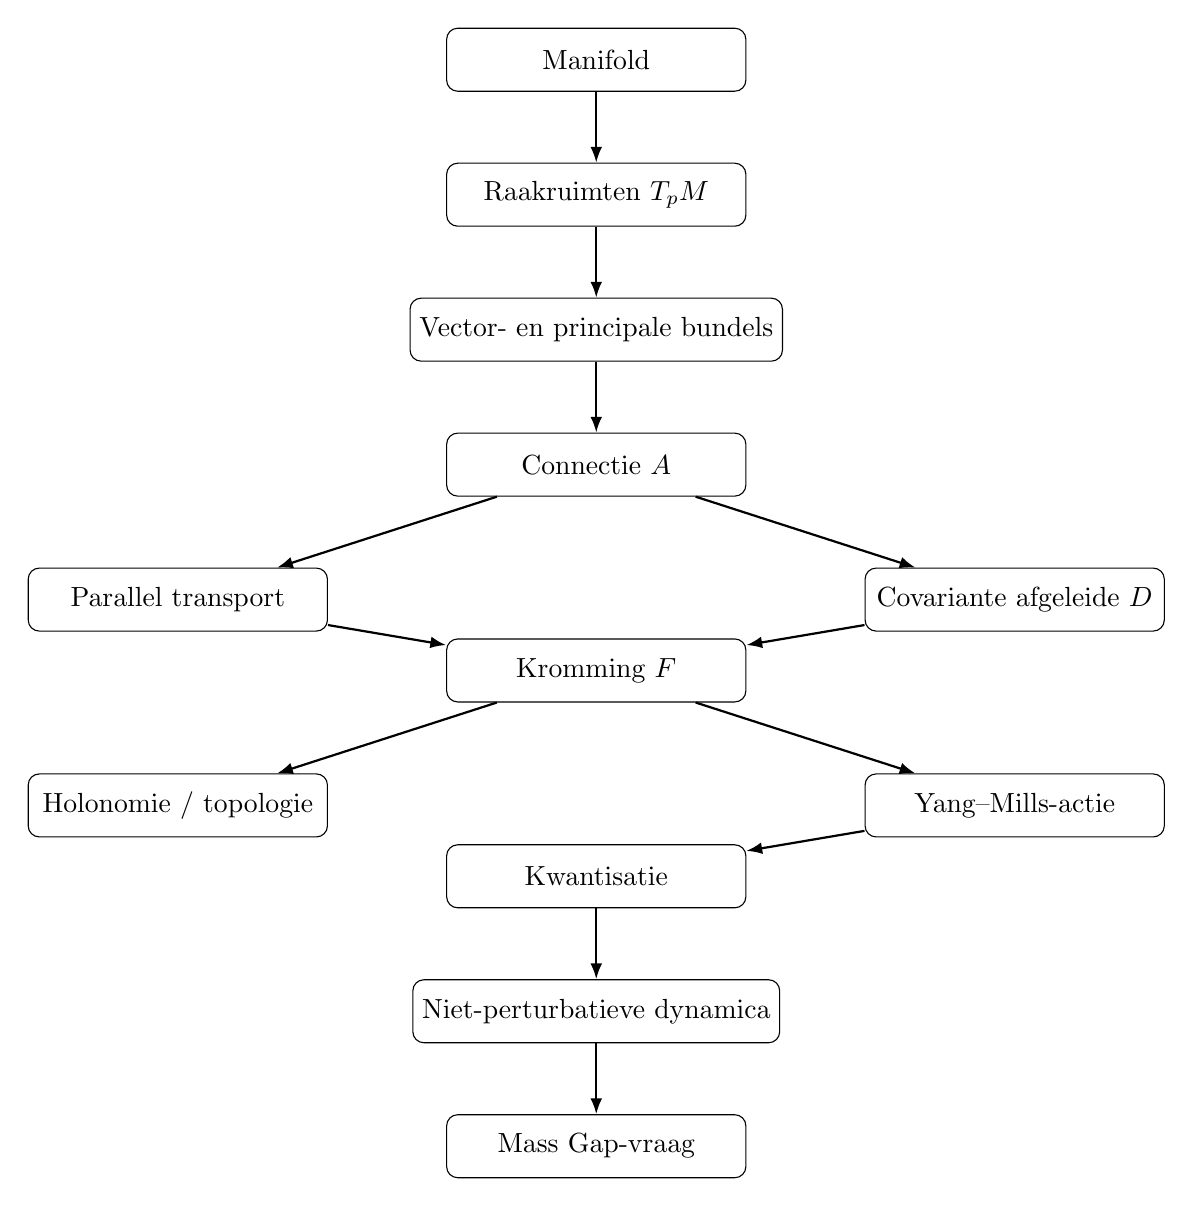
\begin{tikzpicture}[
node distance=9mm and 15mm,
box/.style={draw,rounded corners,align=center,minimum width=38mm,minimum height=8mm},
arrow/.style={-{Latex[length=2mm]},thick}
]
\node[box] (man) {Manifold};
\node[box,below=of man] (tan) {Raakruimten $T_pM$};
\node[box,below=of tan] (bun) {Vector- en principale bundels};
\node[box,below=of bun] (conn) {Connectie $A$};
\node[box,below left=of conn] (pt) {Parallel transport};
\node[box,below right=of conn] (cov) {Covariante afgeleide $D$};
\node[box,below=18mm of conn] (curv) {Kromming $F$};
\node[box,below left=of curv] (top) {Holonomie / topologie};
\node[box,below right=of curv] (ym) {Yang--Mills-actie};
\node[box,below=18mm of curv] (qft) {Kwantisatie};
\node[box,below=of qft] (np) {Niet-perturbatieve dynamica};
\node[box,below=of np] (gap) {Mass Gap-vraag};
\draw[arrow] (man)--(tan);
\draw[arrow] (tan)--(bun);
\draw[arrow] (bun)--(conn);
\draw[arrow] (conn)--(pt);
\draw[arrow] (conn)--(cov);
\draw[arrow] (pt)--(curv);
\draw[arrow] (cov)--(curv);
\draw[arrow] (curv)--(top);
\draw[arrow] (curv)--(ym);
\draw[arrow] (ym)--(qft);
\draw[arrow] (qft)--(np);
\draw[arrow] (np)--(gap);
\end{tikzpicture}
\end{center}

\section{Volledige skilltree van Fase 1 tot Fase 7}

\[
\begin{array}{c}
\text{Getallen en bewerkingen}\\
\downarrow\\
\text{Algebra, functies en geometrie}\\
\downarrow\\
\text{Limieten, afgeleiden en integralen}\\
\downarrow\\
\text{Vectoren, matrices en vectorruimten}\\
\downarrow\\
\text{Complexe getallen, differentiaalvergelijkingen en Fourier}\\
\downarrow\\
\text{Groepen, topologie en tensoren}\\
\downarrow\\
\text{Manifolds en bundels}\\
\downarrow\\
\text{Connecties en kromming}\\
\downarrow\\
\text{Gauge-symmetrie en Yang--Mills}\\
\downarrow\\
\text{Kwantumveldentheorie}\\
\downarrow\\
\text{Mass Gap-vraag}
\end{array}
\]

\section{Samenvatting van Fase 7}

\subsection*{Milestone 7.1 --- Gevectoriseerde Bundels \& Connecties}
Je leerde dat een manifold lokaal Euclidisch is, dat ieder punt een eigen raakruimte heeft en dat zulke lokale vectorruimten samen bundels vormen. Omdat elementen in verschillende fibers niet vanzelf vergelijkbaar zijn, introduceerden we connecties. Parallel transport en covariante afgeleiden zijn manifestaties van die connectie; kromming meet de path-afhankelijkheid van dat transport.

Belangrijkste begrippen:
\begin{itemize}
    \item manifold en kaart;
    \item raakruimte en raakbundel;
    \item vectorbundel en sectie;
    \item differentiaalvormen, $\wedge$, $\dd$ en $*$;
    \item principale bundel en geassocieerde bundel;
    \item connectie, parallel transport en covariante afgeleide;
    \item metriek, Christoffelsymbolen en Levi-Civita-connectie;
    \item kromming en holonomie.
\end{itemize}

\subsection*{Milestone 7.2 --- Yang--Mills Theorie}
Je leerde dat lokale interne symmetrie een gauge-connectie vereist. De kromming van die connectie is de veldsterkte
\[
F=\dd A+A\wedge A.
\]
De natuurlijke gauge-invariante actie is opgebouwd uit
\[
\Tr(F\wedge*F).
\]
Niet-abelse groepen maken de theorie niet-lineair en laten gaugevelden onderling interageren.

Belangrijkste begrippen:
\begin{itemize}
    \item globale versus lokale symmetrie;
    \item gaugegroep en Lie-algebra;
    \item representaties;
    \item gaugepotentiaal en covariante afgeleide;
    \item veldsterkte als kromming;
    \item Yang--Mills-actie en veldvergelijkingen;
    \item Bianchi-identiteit;
    \item Wilson-lussen;
    \item standaardmodel-gaugegroep;
    \item kwantisatie, gauge-fixing, renormalisatie en asymptotische vrijheid.
\end{itemize}

\subsection*{Milestone 7.3 --- Het Begrip}
De afzonderlijke delen vormen nu één patroon:
\[
\text{symmetrie} \to \text{lokale vrijheid} \to \text{bundel} \to \text{connectie} \to \text{kromming} \to \text{dynamica} \to \text{kwantisatie}.
\]

De Mass Gap-vraag ligt aan het uiteinde van deze keten omdat zij niet alleen geometrie of algebra betreft, maar de spectrale structuur van een volledig niet-perturbatieve quantumveldentheorie.

\begin{kernidee}
Het belangrijkste inzicht van het volledige leerpad is niet één formule. Het is dat moderne mathematische fysica ontstaat wanneer algebra, analyse en geometrie elkaar ontmoeten in een theorie van lokale symmetrie.
\end{kernidee}

\section*{Eindbeeld}
\addcontentsline{toc}{section}{Eindbeeld}

Fase 1 begon met de vraag hoe je telt. Fase 7 eindigt met de vraag hoe lokale symmetrieën, geometrische connecties en quantumdynamica samen een fundamentele krachtentheorie kunnen vormen.

De intellectuele route kan worden samengevat als:
\[
\begin{aligned}
\text{getal} &\to \text{variabele} \to \text{functie} \to \text{verandering} \\
&\to \text{vectorruimte} \to \text{dynamisch systeem} \to \text{symmetrie} \\
&\to \text{geometrische structuur} \to \text{gaugeveld} \to \text{quantumveld}.
\end{aligned}
\]

Daarmee is het oorspronkelijke leerpad inhoudelijk gesloten: de elementaire bouwstenen van de eerste fasen zijn uitgegroeid tot de taal waarin Yang--Mills-theorie en de Mass Gap-vraag kunnen worden begrepen.

\end{document}
